\documentclass[10pt,oneside,a4paper,final,english]{memoir}

\usepackage{palatino}
\usepackage{microtype}
\usepackage{lscape}
\usepackage{multicol}
%\usepackage{epic,eepic}
\usepackage{latexsym}
\usepackage{verbatim}
\usepackage{listings}
\usepackage{ulem}
\usepackage{hyperref}

\let\footruleskip\undefined
\usepackage{fancyhdr}
\usepackage[final]{fixme}

\let\fref\undefined
\usepackage[plain]{fancyref}

%% FOR LOOP
\usepackage{ifthen,calc}
\newcounter{myforloopcounter}
\newcommand{\forloop}[5][1]% 
{\setcounter{#2}{#3}% 
\ifthenelse{#4}% 
{#5%
  \addtocounter{#2}{#1}% 
  \forloop[#1]{#2}{\value{#2}}{#4}{#5}% 
}%
% Else 
{}%
}% 


%% USAGE
%\forloop[step]{counter}{initial_value}{conditional}{code_block} 
\usepackage[english]{babel}
\usepackage[utf8]{inputenc}

%\selectlanguage{danish}

\lstset{language=Python,basicstyle=\small,
  columns=fullflexible}


\usepackage[pdftex]{graphicx}

\DeclareGraphicsExtensions{.jpg .png .pdf}


\usepackage{amsmath}
\usepackage{latexsym}
\usepackage{amssymb}


\usepackage[osf,sc]{mathpazo}
\usepackage{microtype}
%\usepackage{fourier}
\linespread{1.05}

%\usepackage[charter]{mathdesign}
%\usepackage{lmodern}

%\usepackage{algorithmic}
%\usepackage{algorithm}

\usepackage{amsthm}


\theoremstyle{plain}  \newtheorem{definition}{Definition}
\theoremstyle{remark} \newtheorem{lemma}{Lemma}
\theoremstyle{plain}  \newtheorem{theorem}{Theorem}
\theoremstyle{remark}  \newtheorem{example}{Example}


\newcommand{\p}{\ensuremath{^\prime}}
\DeclareGraphicsExtensions{.jpg, .eps, .png}
%%% Local Variables:
%%% mode: plain-tex
%%% TeX-master: "../master"
%%% End:

%\usepackage{algorithmic}
\usepackage{algorithm}
\usepackage[sectionbib,square]{natbib}
%\bibpunct{(}{)}{,}{a}{}{}
\setcitestyle{alpha}
%\setcitestyle{numbers,aysep={},yysep={;}}

\usepackage{datetime}

%\chapterstyle{thatcher}

%\setcounter{chapter}{1}
%\setcounter{secnumdepth}{1}
\setcounter{tocdepth}{2}




%\pagestyle{fancy}
\begin{document}
  \fontencoding{T1}
%  \fontseries{m}
%  \fontshape{n}
%  \fontsize{12}{15}
%  \selectfont


%%%%%%%%%%%%%%%%%%%%%%%%%%%%%%%%%%%%%%%%%%%%%%%%%%%%%%%%
%                    Forside
%%%%%%%%%%%%%%%%%%%%%%%%%%%%%%%%%%%%%%%%%%%%%%%%%%%%%%%%
\makeatletter % open mode for reading @ signed variables
\def\maketitle{%
 \null
 \thispagestyle{empty}%
 \vfill
 \begin{center}\leavevmode
   \normalfont
   \LARGE{\raggedleft \@title\par}%
   \hrulefill\par
   \large{\raggedleft \subtitle\par}%
   \vskip 2cm
   {\today\par}%
 \end{center}%
 \vfill
 \begin{flushleft}
   {\large \@author } \\
   {\footnotesize \suplementInfo }
 \end{flushleft}
 \clearpage % Terminates the page here. Everything else vil be placed
            % on next page.
}
\makeatother % closing mode for reading @ signed variables
%%%%%%%%%%%%%%%%%%%%%%%%%%%%%%%%%%%%%%%%%%%%%%%%%%%%%%%%
%               Data til forside
%%%%%%%%%%%%%%%%%%%%%%%%%%%%%%%%%%%%%%%%%%%%%%%%%%%%%%%%
\title{Final Hand In $\cdot$ Week VIII}

\def\subtitle{CCO $\cdot$ Constraint Continuous Optimization}

\author{Johan Sejr Brinch Nielsen} \def\suplementInfo{

\kern 5pt \hrule width 11pc \kern 5pt

\begin{tabular}{ll}
Email: & zerrez@diku.dk  \\
Cpr.:  & 260886-2547
\end{tabular}

% putter 5pt spacing oven over og neden under stregen
\kern 5pt \hrule width 11pc \kern 5pt

Dept. of Computer Science,  \\
University of Copenhagen

}


\maketitle
\newpage

\frontmatter
\tableofcontents
\newpage

\section{Introduction}


\section{Problem 1: Mandatory}
I have filled out the Course Evaluation.


\section{Problem 2: Taylor}
\subsection{Taylor Series}
A Taylor series is a series expansion of a function $f(x) : \mathbb{R}
\rightarrow \mathbb{R}$ in some point $a$. It is given by:
\[ f(x) = f(a) + f'(a)(x-a) + \frac{f''(a)}{2!}(x-a)^2 + \ldots +
\frac{f^{(n)}(a)}{n!}(x-a)^n \]

\subsection{Taylor's Theorem}
Taylor's Theorem states that any real function $f$(where we can derive
the needed derivatives) can be expanded as ($a = 0$):
\[ f(x) = f(0) + x f'(0) + \frac{x^2}{x!}f''(0) + \ldots +
\frac{x^{n-1}}{(n-1)!} f^{n-1}(0) +
\int^x_0{\frac{(x-u)^{n-1}}{(n-1)!}f^{(n)}(u) du}\]

Note the remainder denoted by the integral. Taylor series expansion
are an important tool in optimization, since it can result in a simpler
function (f.x. a quadratic function) which approximates the original
objective function.

\section{Problem 3: Line Search Methods}
The principle behind line search methods is to minimize the objective
function by first computing a descent direction and then an
``appropriate'' step size to jump. Examples of line search methods are
steepest descent and Newton's method.

The Armijo and Wolfe conditions is a set of conditions that restrict
the area the optimization method will consider as ``good''
choices. Line search methods can use the conditions to select a step
size after the step direction has been chosen.

\subsection{Armijo Conditions}
The Armijo conditions are satisfied when:
\[ f(x +\alpha p_k) \leq f(x) + c_1\alpha p^T \nabla f(x) \] Where
$x$ is the current point, $p$ is the descent direction,
$\alpha$ is the step size and $0 < c_1 < 1$ is a constant relaxing the
condition. The result of this condition is that the taken step should
lower the objective value at least as much as what we would have
gotten following a straight line in the same direction. $c_1$ relaxes
the gradient of this direction.

\begin{figure}
\caption{Example of Armijo Back-tracking}
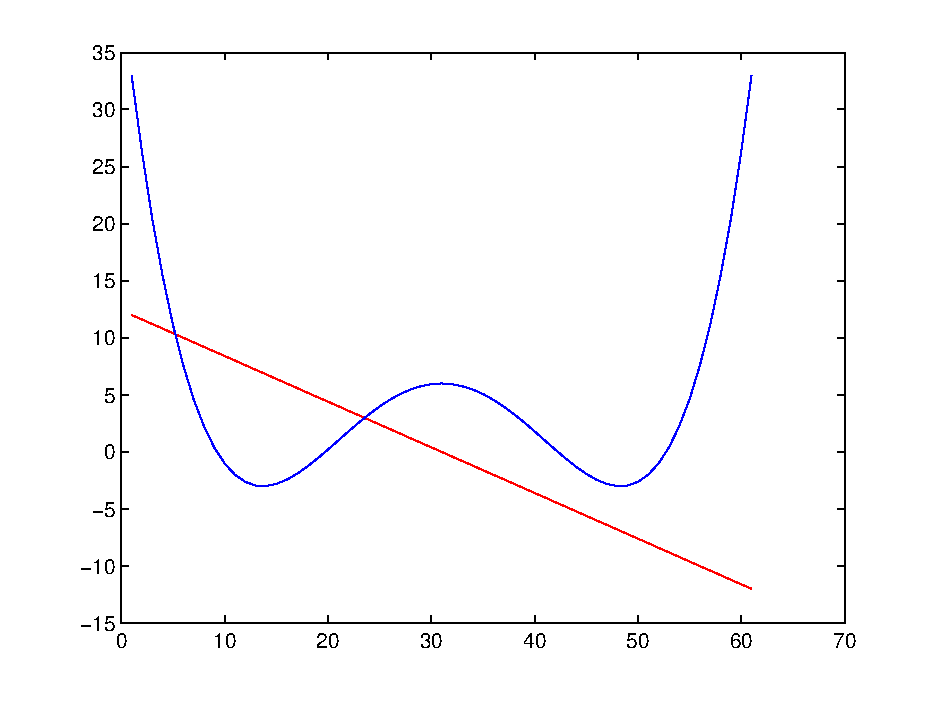
\includegraphics[width=\textwidth]{images/armijo_plot.pdf}
Armijo back-tracking visualized as a line (red) going through a 2D
objection function (blue). Only values beneath the red line is
permitted. The first of the two intersections (to the left) is the
current solution point $x$, while the second denotes the maximum distance
reachable under the conditions.
\end{figure}

\subsection{Wolfe Conditions}
The Wolfe conditions are satisfied when the Armijo conditions are
satisfied and:
\[ p^T \nabla f(x + \alpha p) \geq c_2 p^T \nabla f(x) \] Where $x$ is
the current point, $p$ is the search direction, $\alpha$ is the step
size and $0 < c_1 < c_2 < 1$ is a constant relaxing the condition.

The condition states that the slope of the function in the chosen
point must at least that of the starting point.


\subsection{Armijo Back-tracking}
The projected Armijo back-tracking will, given a search direction $p$,
find a step size $\alpha$ for which $f(x + \alpha p)$ satisfies the
Armijo conditions.

The algorithm starts with a large step length (e.g. 1). The step
length is then lowered until a point that meets the condition is
found.

If the chosen search direction is a descent direction, such a point
must necessarily exist (the condition is satisfied when
$\alpha=0$). However, it may be very close to the initial $x$. If so,
the step taken can be very short, nearly nothing at all. It is
important to ensure a minimum step size to avoid repeating
computations in $x$.

The algorithm can be described with the following pseudo code:
\begin{verbatim}
while not (Armijo-condition of (x+a*c1*pk)) do
  a = a * c
end
\end{verbatim}
Where $0 < c < 1$.


\section{Problem 4: Trust Region Methods}
Trust region methods works by first deciding on a step size and then
compute the a decent direction within the step size (the ``region'').

The idea is to use a model function $m$ that approximates the
objective function $f$. Knowing the step size $\lambda$, the goal is
to find the best search direction in the model function (which is easy
to minimize) and then follow this direction in $f$. Of course one needs
to verify that the model is in fact precise enough to yield a decent
in $f$. If not, the $\lambda$ is lowered. $\lambda$ is a measure for
the precision of the model function. The region containing points with
a distance lower than $\lambda$ away from $x_k$ is called the
``trust'' region.

\subsection{Levenberg-Marquardt}

The Levenberg-Marquardt uses an interpolation between Gauss-Newton and
steepest descent. Intuitively, it tries the direction of Gauss-Newton
and then falls back to steepest descent when unsuccessful.

The Levenberg-Marquardt update value is defined as:
\[ \Delta = - (J^TJ - \lambda I)^{-1} J^T r\]

Where $J$ is the jacobian matrix, $\lambda$ is the step modifier,
$r$ is the residual vector and $\Delta$ is the next modification of
the approximation.
When the step modifier $\lambda$ gets large, it will dominate the
inverted matrix, such that:
\[ \Delta \approx - (-\lambda I)^{-1} J^T r = \]
\[ - \frac{1}{\lambda}I J^T r \]


It is now clear why $\lambda$ becomes a step modifier and how
Levenberg-Marquardt graduately switches to steepest descent.
$\lambda$ determines whether $J^TJ$ or $-\lambda I$ should dominate
the direction. The method adapts both step size and direction during
the optimization, however the step size is always lowered. Hence, it
makes sense to classify this method as a trust region method (bound by
the starting $\lambda$ value).

\subsection{Dogleg}
The Dog-Leg method is based on a combination of the Cauchy point and a
Quasi-Newton method. It uses a second degree Taylor expansion as its
model. It will choose its search direction based on the following
three cases:
\begin{enumerate}
\item When the point suggested by Newton's method is within the trust
  region, this point is selected.
\item If this is not the case and the trust region requests a smaller
  step than that of the Cauchy point, the direction towards this point
  is followed as far as the region permits.
\item In the third case, when the region boundary is between the
  Cauchy point and the Newton point, the intersection between the
  limiting boundary and the line between these two points are chosen.
\end{enumerate}

As can be seen, the possible directions is given by two joined lines
(from $p_k$ to the Cauchy point and further to Newton's point). This
gives a bending line (a ``dog leg''). Note that since the model
function is quadratic, the Newton method will minimize it in a single
iteration. So there is never a need to go further than the point found
by Newton's method.

Specifically, $p_k$ may take one of the following forms:
\begin{enumerate}
\item \[ p_{k+1} = p^B \]
\item \[ p_{k+1} = \frac{\Delta}{\mid p^U\mid}  p^U \]
\item \[ p_{k+1} = p^U + \frac{\Delta - \mid p^U\mid}{
    \mid p^B\mid + 2p^{U\prime} p^B} p^B \]
\end{enumerate}


Where $\Delta$ is the size of the trust region, $p^B$ is the point
suggested by Newton's method and $p^U$ is the Cauchy point. The two
latter points are defined as:
\[ p^B = -B^{-1} \cdot g \]
\[ p^C = \frac{g' g}{g'Bg} \cdot g \]

Where $g$ is the gradient in the point $x_k$, $B$ is an approximation
of the Hessian and $B^{-1}$ is an approximation of its inverse; both
$B$ and $B^{-1}$ are positive definite matrices.

There is one detail in the algorithm yet to be discussed. That is what
size to choose for $\lambda$ and how to adjust this
dynamically. Generally, one should lower $\lambda$ when no decent
direction is found and only raise $\lambda$ when the step taken is as
long as $\lambda$ (the step is restricted by $\lambda$). One way to
achieve this is by comparing the actual improvement in the objective
function with that of the model (the expected improvement).


\section{Problem 5: First Order Optimality Conditions}
The Karush-Kuhn-Tucker (KKT) conditions are a set of \textit{necessary}
conditions that must be satisfied before $x$ can be a minimum of
the function $f$. If the KKT conditions are not satisfied, one can
be sure that $x$ is not a minimum. However, whenever they are
satisfied, one only knows that $x$ \textit{might} be a minimum.

Consider the minimization problem:\\
\begin{center}\begin{tabular}{rl}
$\min_{x}$ & $f(x)$ \\
subject to: & $c(x) \geq 0$
\end{tabular}\end{center}

Where $x \in R^n$, $c$ are the constraints and $f : \mathbb{R}^n
\to \mathbb{R}^n$.

I will now derive the KKS conditions for this minimization problem.
Let us first examine the first-order Taylor expansion of the objective
and constraint function. To maintain feasibility we require that
$c(x+d)=0$, where $d$ is the direction. Hence,
\[ 0 \leq c(x+d) \approx c(x) + \nabla c(x)^T d = c(x)^Td \]
The last step is due to $c(x) = 0$. When this condition is satisfied,
we maintain feasibility after the step in direction $d$.

To ensure an improvement in the objective function, we seek to satisfy
the condition:
\[ 0 > f(x + d) - f(x) \approx \nabla f(x)^T d\]

That is, the objective value should drop when moving in the direction
of $d$ (a descent direction). This is called an improvement to first
order.

Consider the direction $d$ pointing towards a constraint boundary. In
such a case, where the optimal solution is bounded by one or more
constraints, the gradient of $f$ and that of $c$ must be
parrallel. Hence,
\[ \nabla f(x) = \lambda \nabla c(x),\ \lambda > 0\]

When the descent direction is not restricted by any constraints,
normal optimization techniques can be used. Note however, that the
minimzer may lie far from any constrainting boundary that $d$ is
trying to cross.


Considor now the Lagrangian function:
\[ \Lambda (x, \lambda) = f(x) - \lambda c(x) \]

And its derivate:
\[ \nabla_x \Lambda(x, \lambda) = \nabla f(x) - \lambda \nabla
c(x) \]

It is clear that the condition of $\nabla f$ can be written as:
\[ \nabla f(x) = \lambda \nabla c(x) \Rightarrow
   \nabla_x \lambda(x, \lambda) = 0 \]

This is interesting, since it shows a connection between stationary
points in $\Lambda(x, \lambda)$ and possible minimizers in $f$.

A necessary condition for a minimizer $x^\star$ of $f$ is then:
\[ \nabla_x \Lambda(x^\star, \lambda^\star) = 0,\ \lambda^\star \geq
0 \]

Furthermore, we know that the constraints should be fulfilled:
\[c(x^\star) \geq 0\]

However, since this was derived from \textit{active} constraints
(those that limit the search direction), we also require:
\[ \lambda^\star c(x^\star) = 0 \]

This condition ensures either $\lambda^\star$ or $c(x^\star)$ to be
zero. The idea is, that whenever $c(x^\star) > 0$ (we are not near a
constraint boundary) then $\lambda^\star = 0$ and the stationary point
condition reduces to $\nabla f(x^\star) = 0$. On the other hand, having
$c(x^\star) = 0$ allows $\lambda^\star$ to take a negative value.

The Karush-Kuhn-Tucker conditions describe these conditions using sets
$E$ and $I$, where $E$ contains all active constraints and $I$
contains all inactive constraints:
\begin{center}\begin{tabular}{rl}
$ \nabla \Lambda(x^\star, \lambda^\star) = 0,$ & \\
$  c_i(x^\star) = 0, $ & for all $i \in E,$ \\
$  c_i(x^\star) \geq 0,$ & for all $i \in I,$ \\
$ \lambda_i^\star \geq 0,$ & for all $i \in I$, \\
$ \lambda_i^\star c_i(x^\star) = 0,$ & for all $i \in E \cup I$
\end{tabular}\end{center}


\section{Problem 6: Calculus of Variation}
Given the functional:
\[ S = \int_a^b \Lambda (x, f, f')\ dx\]
The Euler-Lagrange equation becomes:
\[ - \frac{d}{dx}\frac{\rho L}{\rho f'} + \frac{\rho L}{\rho f} = 0 \]


\section{Problem 7: Linear Complementary Problem}
A linear complimentary problem (LCP) is a specific category of
problems, which take the form:\\

\begin{center}\begin{tabular}{rl}
$A\lambda + b$ & $\geq 0$ \\
$\lambda$ & $\geq 0$\\
$\lambda^T (A\lambda + b)$ & $= 0$
\end{tabular}\end{center}

Where $A$ is a given matrix, $b$ is a given vector and $\lambda$ is
the solution vector that is to be found.


\subsection{Connection to Constrained Optimization}
Any LCP can be reformulated as a quadratic problem (QP). The QP
corresponding to the LCP in the previous section becomes:
\begin{center}\begin{tabular}{rrl}
$\min_\lambda$ & $\lambda^T(A\lambda+b)$ & \\
such that: & $A\lambda + b$ & $\geq 0$ \\
           & $\lambda $ & $\geq 0$
\end{tabular}\end{center}

Since $z\geq 0$ and $Mz+q\geq 0$, the product $z^T(Mz+q)$ must be
positive. Hence, the minimum must be $0$. The inequality constraints
are still maintained, so the optimal solution will be equal to that of
the original LPC.

\subsection{Algebraic Transformation from LCP to QP}
In this section I will convert the LCP solved in this weeks assignment
to an QP. Let's start with the original LCP:
\begin{center}\begin{tabular}{rl}
$A\lambda + b$ & $\geq 0$ \\
$\lambda$ & $\geq 0$\\
$\lambda^T (A\lambda + b)$ & $= 0$
\end{tabular}\end{center}

Letting $h(\lambda) = A\lambda + b$, $x^\star = \lambda$ and $y^\star
= h(\lambda)$ we obtain the following reformulation of the
conditions:
\begin{center}\begin{tabular}{rl}
$h(\lambda)$ & $\geq 0$ \\
$\lambda$ & $\geq 0$\\
$\lambda^T h(\lambda)$ & $= 0$\\

$(x^\star)^T h(\lambda)$&$= 0$
\end{tabular}\end{center}

The new conditions (last three) being repetitions of the original
conditions (first three). Since $\min(\lambda, y^\star = A\lambda+b) =
0$ (see Splitting Method, page \pageref{splitting}) we can add the
constraint:
\begin{center}\begin{tabular}{rl}
    $(y^\star)^T \lambda $&$= 0$
\end{tabular}\end{center}

Furthermore, since $x = \lambda$ and $y^\star = h(x)$ the following
constraint is valid:
\[ h(\lambda) + \nabla h(\lambda)^T \lambda - \nabla h(\lambda)^T
\lambda - h(\lambda) = 0 \Rightarrow\]
\[ h(\lambda) + \nabla h(\lambda)^T \lambda - \nabla h(\lambda)^T
x^\star - y^\star = 0 \]

The full set of conditions is now:
\begin{center}\begin{tabular}{rl}
$h(\lambda)$ & $\geq 0$ \\
$\lambda$ & $\geq 0$\\
$\lambda^T h(\lambda)$ & $= 0$\\

$(x^\star)^T h(\lambda)$&$= 0$ \\

$(y^\star)^T \lambda $&$= 0$ \\

$h(\lambda) + \nabla h(\lambda)^T \lambda - \nabla h(\lambda)^T
x^\star - y^\star $&$= 0$
\end{tabular}\end{center}

Which are the first order optimality conditions for the QP
\begin{center}\begin{tabular}{rrl}
$\min_\lambda$ & $\lambda^T h(\lambda)$ & \\
such that: & $h(\lambda)$ & $\geq 0$ \\
           & $\lambda $ & $\geq 0$
\end{tabular}\end{center}

This transformation to QP shows that it is possible to solve LCP's
using QP methods. An alternative way of showing this is to derive the
KKT conditions from a QP and show that these reduce to an LCP.


\section{Problem 8: Splitting Method}
\label{splitting}
The Splitting method solves a LCP by first splitting the matrix $A$ in
two. Hereafter, it defines a series of sub-problems which also belongs
to the LCP class. However, hopefully these are easy to solve.

The first step is to split $A$ into to new matrices $M$ and $N$ such
that:
\[ A = M - N \]

The sub-problem is now defined as:
\begin{center}\begin{tabular}{rl}
$M\lambda^{k+1} + c^k$ & $\geq 0$ \\
$\lambda^{k+1}$ & $\geq 0$\\
$(\lambda^{k+1})^T (M\lambda^{k+1} + c^k)$ & $= 0$
\end{tabular}\end{center}

Where $c^k = b - N\lambda^k$. Letting $M\lambda^{k+1}$ be $M\lambda^k$
makes the left-hand side of the first inequality become:
\[ M \lambda^k + c^k = M\lambda^k + b - N\lambda^k \]
\[ = A\lambda^k + b\]

And the sub-problem is back to the original LCP. Hence, the only
difference lies in using $\lambda^{k+1}$ together with $M$ and
$\lambda^k$ together with $N$. Since $\lambda^k$ is the approximation
of $\lambda^\star$ at iteration $k$, and $\lambda^{k+1}$ that at
iteration $k+1$, this is a fixed point computation yielding a solution
to the original LPC.

Not surprisingly, this fixed point iteration can be solved
iteratively. A bit more surprising is, that we need to apply the
minimum map reformulation. This reformulation yields the following
root-search problem:
\[ \min (\lambda^{k+1}, M\lambda^{k+1} + c^k) = 0 \]
This formulation ensures the inequality constraints are fulfilled,
since neither can be negative (the smallest of the two must be
$0$). This is equivalent to the equality constraint, that ensures the
product of the two is $0$. Hence, the new formulation is the same
as the sub-problem.

We can now work on the new formulation:
\begin{center}\begin{tabular}{rlll}
    $ \min $ & $(\lambda^{k+1}, M\lambda^{k+1} + c^k)$&
    $ = 0 $ & $\Rightarrow $ \\

    $ \min $ & $(0, M\lambda^{k+1} + c^k - \lambda^{k+1}) $&
    $= -\lambda^{k+1} $ & $\Rightarrow $ \\

    $ \max $ & $(0, - M\lambda^{k+1} - c^k + \lambda^{k+1}) $&
    $= \lambda^{k+1} $ &
\end{tabular}\end{center}

The result is a fixed point problem (it contains $\lambda^{k+1}$ on
both sides). However, there is one more trick up the sleeve: case
analysis on the sign of the $i$th element of $S = -M\lambda^{k+1} - c^k +
\lambda^{k+1}$:

\paragraph{Case 1: } $S_i = (-M\lambda^{k+1}-c^k+\lambda^{k+1})_i < 0$\\
If this is the case $\lambda^{k+1}_i = 0$, since $0 > S_i$.

\paragraph{Case 2:} $S_i = (-M\lambda^{k+1}-c^k+\lambda^{k+1})_i \geq 0$\\
Clearly $S_i = \lambda^{k+1}_i$, since $S_i > 0$. That is:
\[ (-M\lambda^{k+1}-c^k+\lambda^{k+1})_i = \lambda^{k+1}_i \Rightarrow \]
\[ (-M\lambda^{k+1}-c^k)_i = 0 \Rightarrow \]
\[ (-M\lambda^{k+1})_i = c^k_i \]

This situation is interesting. $\lambda^{k+1}_i$ is now present on the
left hand side only. Assuming that $M$ is reversible, we can compute
$\lambda^{k+1}$ as:
\[ \lambda^{k+1}_i = (-M^{-1}c^k)_i = (-M^{-1}(b - N\lambda^k))_i \]

Combining the two cases yields the following closed term for
$\lambda^{k+1}$:
\[ \lambda^{k+1} = \max(0, M^{-1}N\lambda^k - b) \]

In order to solve the LCP, one can approximate on $\lambda^\star$
using above equation until an acceptable error has been reached.


\section{Problem 9: Reformulation}
This problem reminds me of the tasks in Inverse Kinematics. Here we
had a function $F : \mathbb{R}^n \to \mathbb{R}^m$, transforming
$n$ angles into a point of $m$ dimensions. The goal was to minimize
the distance to a specifif $m$-dimensional point $e$. A function $f :
\mathbb{R}^n \to \mathbb{R}$ was defined by:
\[ f(\theta) = (F(\theta) - e) \cdot (F(\theta) - e) \]

That is, $f$ is a measure for the distance from the point given by the
angles in $\theta$ to the wanted end point. The minization problem can
now be formulated as:
\begin{center}\begin{tabular}{rl}
$\min_\theta$ & $f(\theta)$
\end{tabular}\end{center}

I believe this is an example of the transformation wanted in this task.


\section{Problem 11: Problem Modeling}
In this section, I will go through the problems solved during this
course and how they were modelled in the world of optimization.

The first framework we used was designed to solve Inverse Kinematics
problems. In this case, the problem of finding $n$ angles that would
make an arm reach a chosen point. An $F : \mathbb{R}^n \to
\mathbb{R}^m$ function from angles to coordinates was given. The goal
was now to find $\theta$ that would solve the non-linear equation
$F(\theta) - e = 0$. Using this the objective function $f :
\mathbb{R}^n \to \mathbb{R}$ was defined as the distance from the
point reached through the found angles to the chosen end point
$e$. The function $f$ could now be optimized using unconstained
minimization methods.

To make things more interesting, a few constraints was added to the
problem. The angles in $\theta$ was limited to a fixed interval, hence
adding inequality constaints of the form $l \leq \theta \leq u$. The
model would have to ensure, that the found solution was inside this
boundary. Fortunately, this was quite simple, due to the box-property
of the inequality (the constraints form a ``box'' around the feasible
region). I experimented with allowing some of the angles to be loose,
by not enforcing the constraints on these, and with tightening the
permitted range bit by bit. This was the inspiration for some very
interesting animations.

Hereafter, we moved on to physics simulation of bouncing balls. This
was modelled mathematically with respect to the physical rules that
were present in the simulation. The result was a linear
complimentarity problem, that seeked to minimize the physical energy
present in the system. Constraints were added whenever two balls
collided and removed as soon as they were distanced again. Combined
with rules of acceleration, this formed the basis for the simulation.

Lately, we have looked at Calculus of Variations, where the functions
plays the role part instead of $n$-dimensional vectors. An example of
such an optimization problem is to find the function, who's
function-line between points $a$ and $b$ travel the shortest
distance. The optimal solution is of course a straight line ($f(x) =
ax+b$ in 2-dimensions), but it is a simple example in a series of
complex optimization problems.



\section{Absense}
I have noted, that I have gained 1 absent mark. I do not recall being
absent a full monday $\ldots$



\end{document}

%%% Local Variables:
%%% mode: latex
%%% TeX-master: t
%%% End:
